\documentclass[11pt, a4paper, oneside, openright]{article}
\usepackage{float}
\usepackage{url}
\usepackage[acronym]{glossaries}
\usepackage[style=ieee]{biblatex}
\addbibresource{references.bib}

\newacronym{hci}{HCI}{Human-Computer Interaction}
\newacronym{acm}{ACM}{Association for Computing Machinery}
\newacronym{ieee}{IEEE}{Institute of Electrical and Electronics Engineers}

\newfloat{fig}{thp}{lof}[section]
\floatname{fig}{Figure}

\title{Project Title}
\author{Liam Fenneman}

\usepackage[image,ecs]{vuwproject} 

% \supervisor{}
\otherdegree{Bachelor of Engineering with Honours}
\date{}

\begin{document}

\frontmatter

\begin{abstract}
    This document gives some ideas about how to write a project proposal, and
    provides a template for a proposal. You should discuss your proposal with
    your supervisor. When writing the abstract (this part), you will need to
    include the following information at the minimum: (\textit{i}) the problem
    you are solving and why it matters [1-2 sentences]; (\textit{ii}) how you
    plan to solve the problem, including the resources you will need [1-3
    sentences]; and (\textit{iii}) expected output(s) of your project and how
    you plan to test and evaluate them [1-2 sentences]. For this proposal, the
    abstract should be a single paragraph and should contain 150-250 words.
\end{abstract}

\maketitle

\tableofcontents
\listof{fig}{Figures}

\mainmatter

\section{Introduction}

\begin{figure}[h]
    \centering
    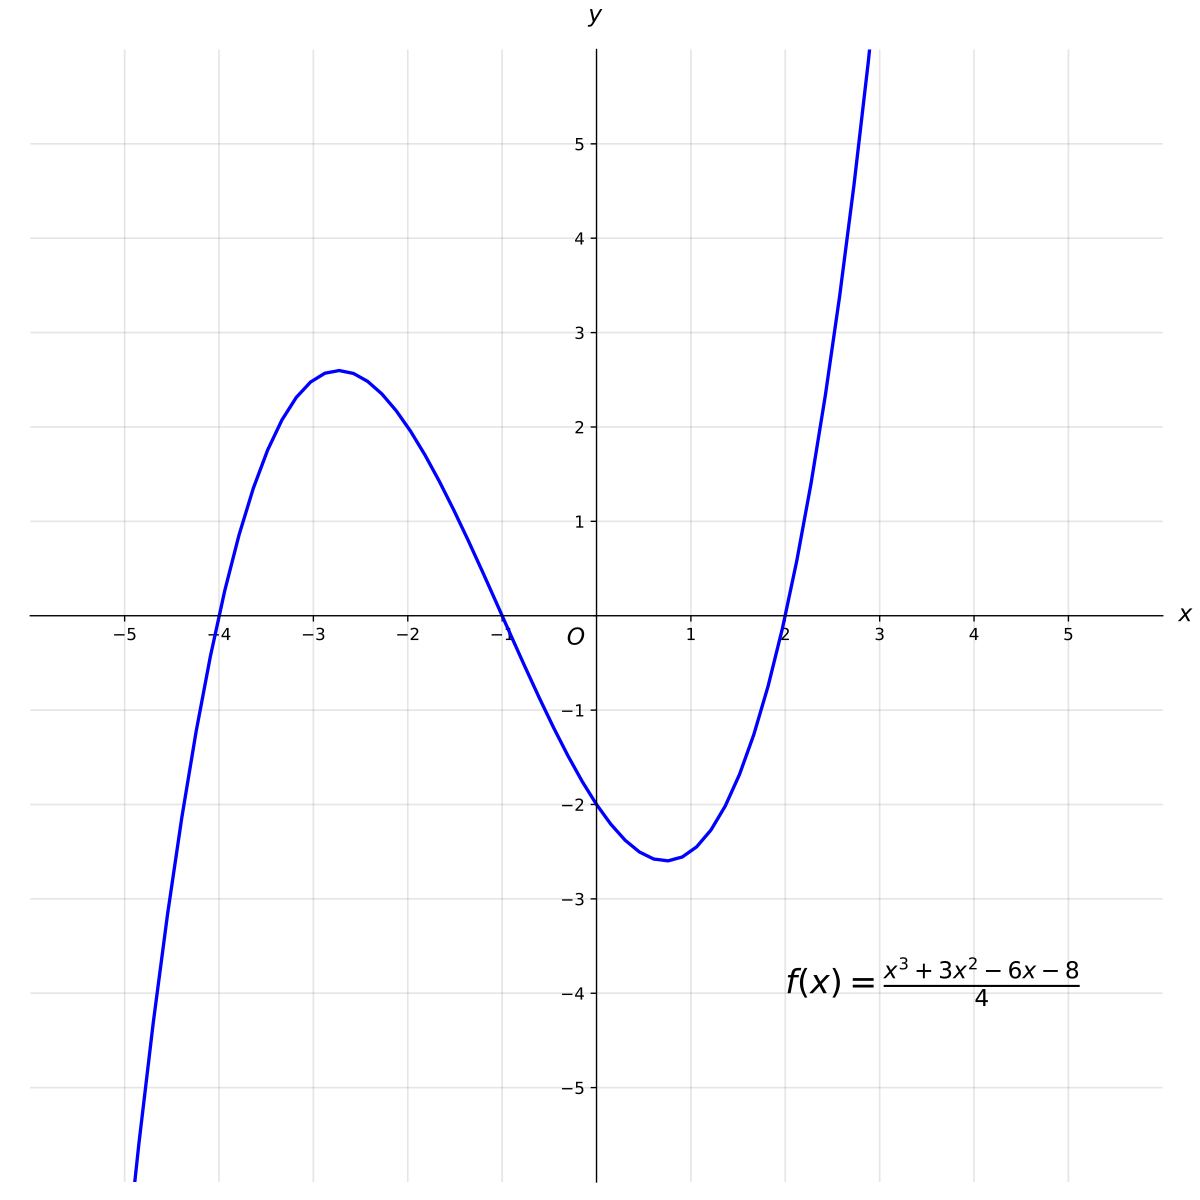
\includegraphics[width=0.75\textwidth]{images/example}
    \caption{Example image. Source: \cite{example}}
    \label{fig:example}
\end{figure}

You can reference Figure \ref{fig:example} like this.

In this section you should include a very brief introduction to the problem and
the project.

Your project proposal should cover the following points:

\begin{itemize}
\item the engineering problem that you are going to solve;
\item how you plan to solve your problem;
\item how you intend to evaluate your solution; and
\item any resource requirements for your project such as software,
  hardware or other resources that will be needed in the course of the project.
\end{itemize}

\textbf{Your proposal should be not more than than 8 pages long.} 

\section{The Problem}

In this section you should give a brief description of the problem itself. You
want to briefly explain the problem, why it is important to solve the problem
and define your project aims. After reading this section, the reader should
understand why it is a problem, believe that it is important to solve and have a
clear idea of the aims of your project.

When describing the aims of the project, you should avoid vague, unmeasurable
words like `analyse', `investigate', `describe', and use specific, measurable
words like `implement', `demonstrate', `show', `prove'.

For example:

\begin{description}
    \item[Good] The aim of this project is to implement and evaluate a
        management system for network switches;
\end{description}
is much better than:
\begin{description}
    \item[Bad] The aim of this project is to investigate management systems for
        network switches.
\end{description}

In the second case there is no idea of how much work is involved, and you will
never know whether you have finished. You and your supervisor (and the markers
of your project) may have very different ideas about what such an
`investigation' involves. Of course, it is possible that the task you set
yourself is not achievable, but if you are clear from the outset this is less
likely, and will more easily be corrected.

\section{Proposed Solution}

In this section you will explain how you plan to solve the problem, that is, how
you intend to carry the project out. At this early stage you need to be both
clear about what you are going to do and flexible enough to adapt to changing
circumstances. Making an early plan will not prevent you from running into
trouble, but it will help you identify possible problems early. For example, if
you intended to run an experiment in \gls{hci}, you might realise early on that
there would be problems gathering sufficient data to get reliable results, and
that you should re-design your experiment.

Part of the planning process involves producing a timetable for when the work is
actually going to be done.

Each part of the project should produce some output. For example you might plan
on spending two weeks on background reading: the output of this will be a
bibliography, and a possibly a literature survey for your report. Indeed, if you
take the advice given above about having specific, measurable goals, you should
describe this part of your project as:

\begin{description}
\item[Good] Produce bibliography (est: 2 weeks)
\end{description}
rather than
\begin{description}
\item[\bf Bad] Background reading (est: 2 weeks)
\end{description}

Note that the methodology you outline here is dependent upon the type of project
and engineering area. You must talk to your supervisor about this.

\section{Evaluating your Solution}

In this section you will explain how you will evaluate your solution once you
have built it. The method of evaluation will be domain specific. Your supervisor
should provide guidance as to what is an appropriate form of evaluation. For
example, user testing for a \gls{hci} project or performance measurement for a
Network Engineering project.

\section{Resourcing and Ethics}

In this section you will detail any resource requirements such as hardware,
software or access. You should address each of these points, even if only to
indicate that they are not of particular concern to your project.

\subsection{Hardware}

Discuss the hardware components that your project will be using. You need not
include the computers that you will be using to carry out the development,
unless your project requires specialised computer hardware to do this part.
Example hardware components are machines, lab instruments, musical instruments,
robots, drones, servers, mobile devices, single-board computers, sensors,
actuators, circuits and circuit components, network equipment, solar panels,
batteries, enclosures, mounting poles, etc.  

\subsection{Software, Datasets and Models}

Discuss the specialised software (applications, compilers, libraries,
development kits, simulators, solvers, etc) to be used. You need not include
common desktop software such as browsers, office applications, IDEs, and
editors. This is also the place to mention datasets and models that you plan to
use. 

\subsection{Space, Virtual Resources and Access}

Discuss the space (for instance labs or specialised rooms, outdoor fields) and
resources that can be accessed virtually (for instance computing grid, virtual
machines, network testbeds) that your project will use, and how you plan to
obtain access them. 

\subsection{Budget}

Provide an estimate of the budget for the project. If the budget is more than
\$500 you should indicate any sources of funding outside the normal ENGR 489
budget. The purchase of special tools or software etc. may not need to be
included in your \$500 limit, however, if something is necessary for your
project you should definitely list it here.

Do not pad the budget to get it up to \$500.

\subsection{Ethics}

Are there ethical considerations with the design or the evaluation of your work?
For example, there may be constraints on the possible set of solutions that you
could explore. If you want to undertake user testing of your system, then you
will need human ethics approval.

\subsection{Safety}

Discuss key health and safety aspects of your project. Note that you will still
need to fill up the appropriate Health and Safety documents.

\subsection{Intellectual Property}

Discuss intellectual property with potential commercial value that might be
developed in the project. See the Handbook for more information regarding IP
agreements.  

\backmatter

\printbibliography

\end{document}
